\documentclass[10pt,twocolumn,letterpaper]{article}

\usepackage{cvpr}
\usepackage{times}
\usepackage{epsfig}
\usepackage{graphicx}
\usepackage{amsmath}
\usepackage{amssymb}
\usepackage{mathrsfs}
\usepackage{mathtools}
\usepackage{subfigure}
\DeclareMathOperator*{\argmin}{arg\,min}
% Include other packages here, before hyperref.

% If you comment hyperref and then uncomment it, you should delete
% egpaper.aux before re-running latex.  (Or just hit 'q' on the first latex
% run, let it finish, and you should be clear).
\usepackage[breaklinks=true,bookmarks=false]{hyperref}

\newcommand{\deva}[1]{\textcolor{red}{[Deva: #1]}}
\newcommand{\songfan}[1]{\textcolor{blue}{[Songfan: #1]}}

\cvprfinalcopy % *** Uncomment this line for the final submission

%\def\cvprPaperID{1627} % *** Enter the CVPR Paper ID here
\def\httilde{\mbox{\tt\raisebox{-.5ex}{\symbol{126}}}}

% Pages are numbered in submission mode, and unnumbered in camera-ready
%\ifcvprfinal\pagestyle{empty}\fi
\begin{document}

%%%%%%%%% TITLE
\title{DAG-CNNs for multi-scale recognition}

\author{Songfan Yang\\
College of Electronics and Information Engineering,\\
Sichuan University, China\\
{\tt\small syang@scu.edu.cn}
% For a paper whose authors are all at the same institution,
% omit the following lines up until the closing ``}''.
% Additional authors and addresses can be added with ``\and'',
% just like the second author.
% To save space, use either the email address or home page, not both
\and
Deva Ramanan\\
Deptment of Computer Science,\\
University of California, Irvine, USA\\
{\tt\small dramanan@ics.uci.edu}
}

\maketitle
%\thispagestyle{empty}

%%%%%%%%% ABSTRACT
\begin{abstract}
We explore multi-scale convolutional neural nets (CNNs) for image classification. Contemporary approaches extract features from a single output layer. By extracting features from multiple layers, one can simultaneously reason about high, mid, and low-level features during classification. The resulting multi-scale architecture can itself be seen as a feed-forward model that is structured as a directed acyclic graph (DAG-CNNs). %We show that DAG-CNNs are just as fast as chain-structured CNNs in terms of training and testing. In fact, training is easier because multi-scale connections tend to minimize the vanishing gradient problem. 
We use DAG-CNNs to learn a set of multiscale features that can be effectively shared between coarse and fine-grained classification tasks. While fine-tuning such models helps performance, we show that even ``off-the-self'' multiscale features perform quite well. We present extensive analysis and demonstrate state-of-the-art classification performance on three standard scene benchmarks (SUN397, MIT67, and Scene15). %and show  state-of-the-art classification performance on all benchmarks., %\ie 55.5\% on SUN397, 76.1\% on MIT67, and 92.4\% on Scene15.
%\ie 56.2\% on SUN397, 77.5\% on MIT67, and 92.9\% on Scene15. 
In terms of the heavily benchmarked MIT67 and Scene15 datasets, our results reduce the lowest previously-reported error by {\bf 23.9\%} and {\bf 9.5\%}, respectively.
\end{abstract}

%%%%%%%%% BODY TEXT
\section{Introduction}


\begin{figure}[t!]
\centering
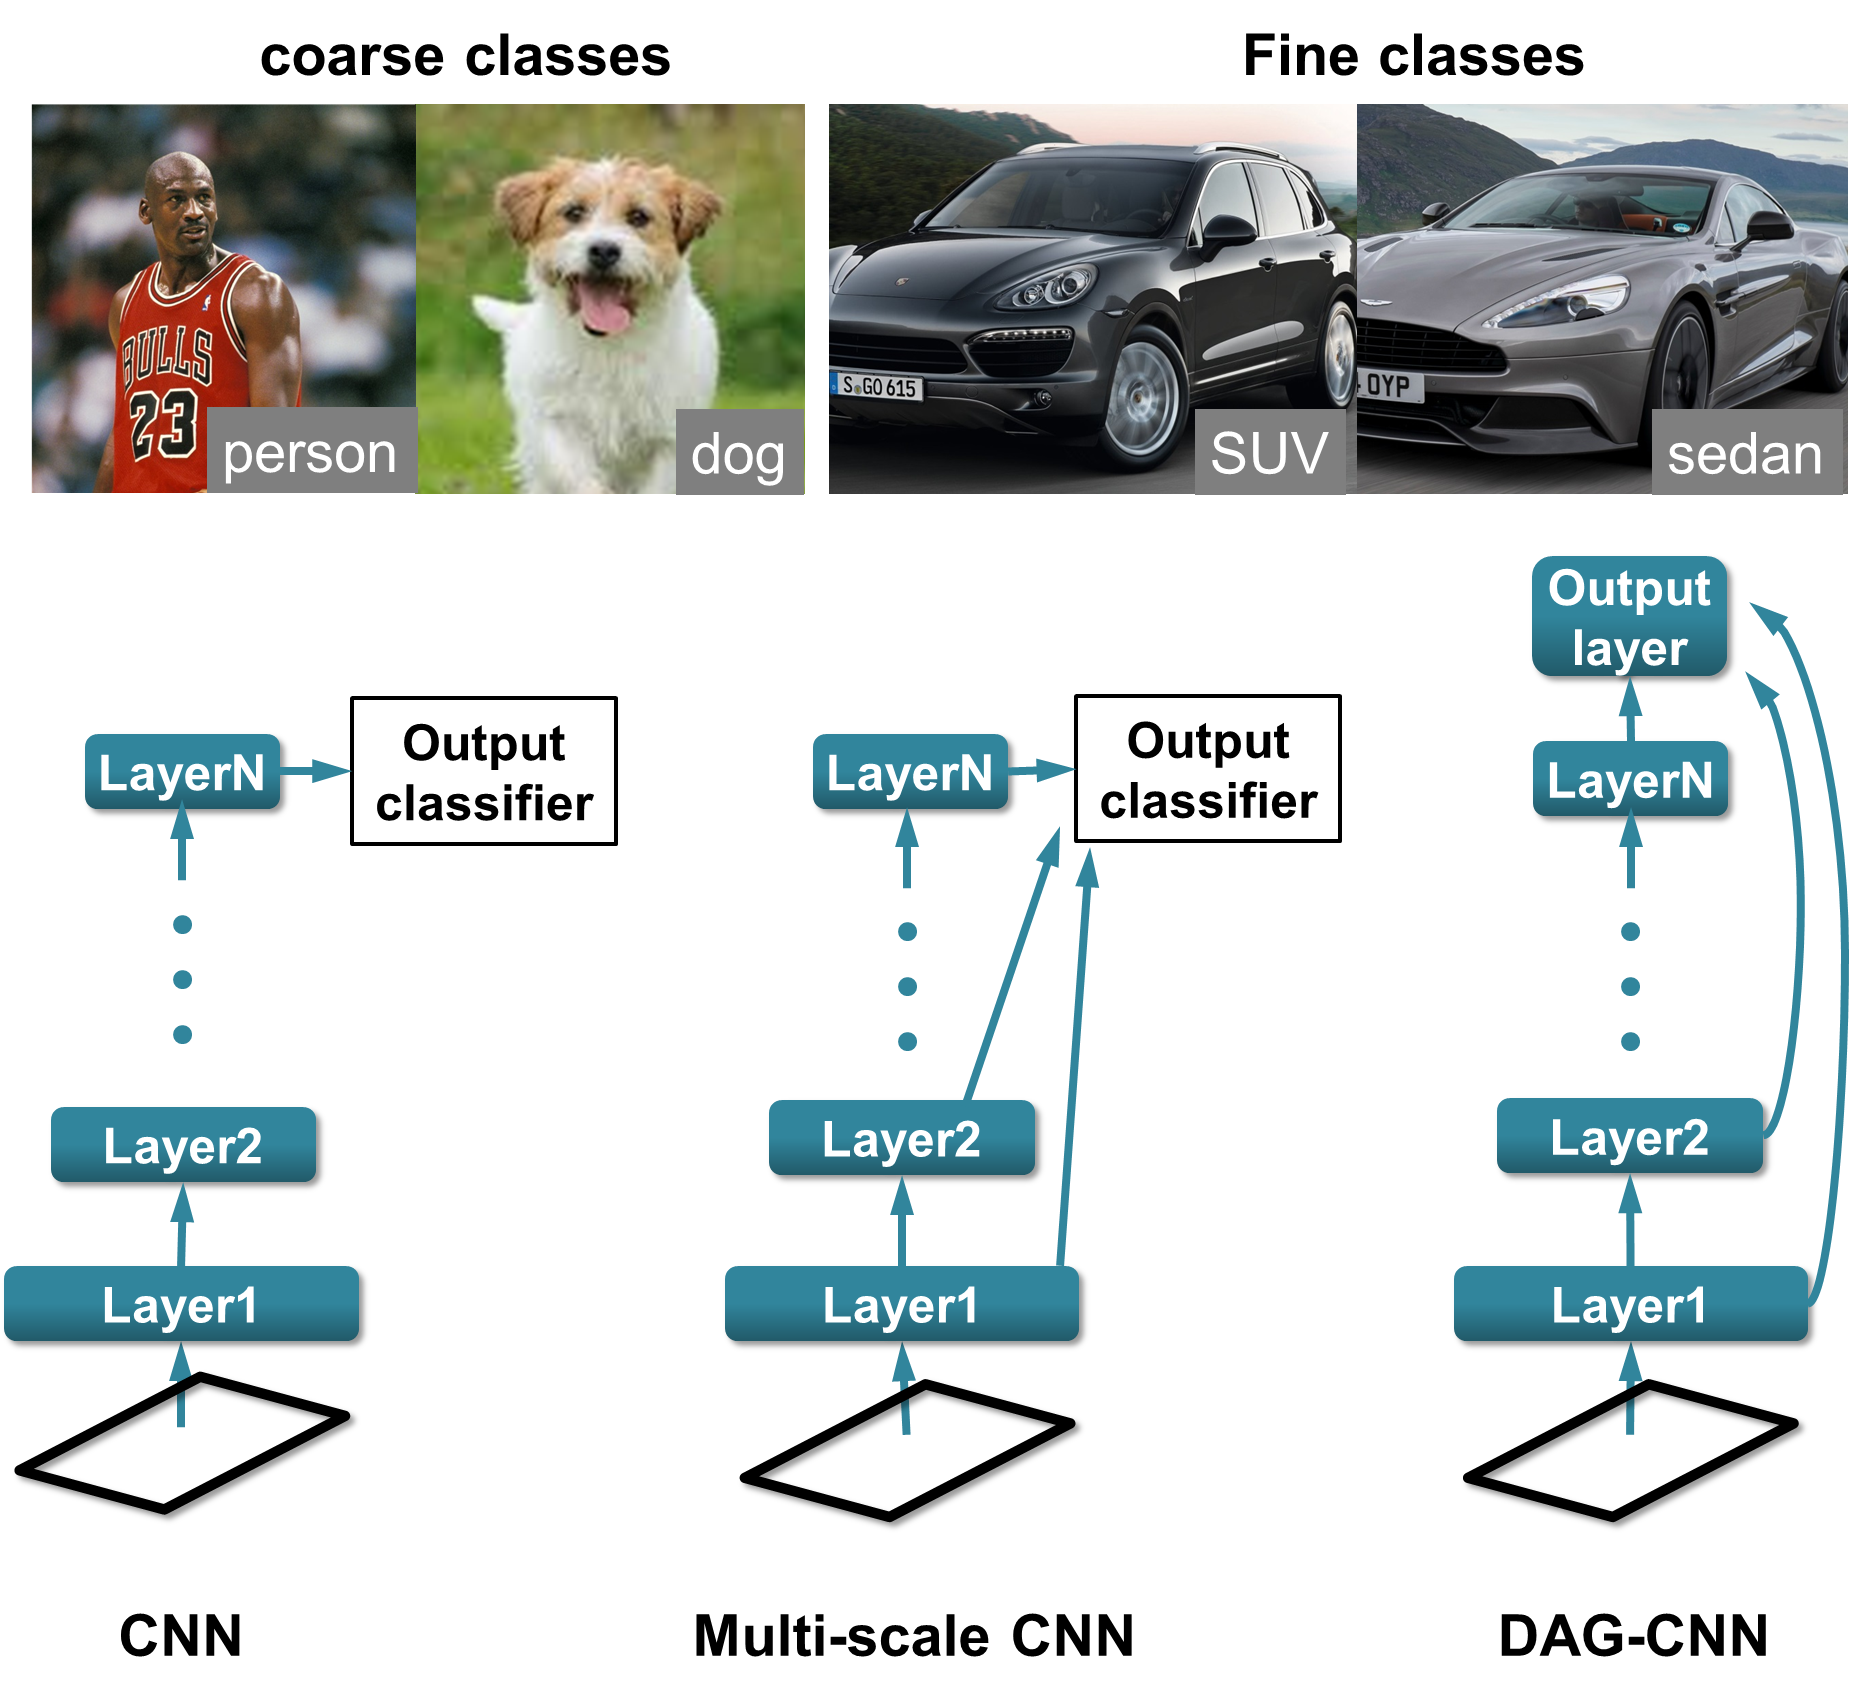
\includegraphics[width=\columnwidth]{fig/splash}
\caption{Recognition typically require features at multiple scales. Distinguishing a person versus dog requires highly invariant features robust to the deformation of each category. On the other hand, fine-grained recognition likely requires detailed shape cues to distinguish models of cars ({\bf top}). We use these observations to revisit deep convolutional neural net (CNN) architectures. Typical approaches train a classifier using features from a single output layer ({\bf left}). We extract multi-scale features from multiple layers to simultaneously distinguish coarse and fine classes. Such features come ``for free'' since they are already computed during the feed-forward pass ({\bf middle}). Interestingly, the entire multi-scale predictor is still a feed-forward architecture that is no longer chain-structured, but a directed-acyclic graph (DAG) ({\bf right}). We show that DAG-CNNs can be discriminatively trained in an end-to-end fashion, yielding state-of-the-art recognition results across various recognition benchmarks. % DAG-CNNs address some well-known challenges with CNNs such as ``vanishing gradients''~\cite{bengio1994learning}. Lower layers in a DAG-CNN still receive a strong gradient signal during learning because they are directly tied to the output layer, making them easier to train.
\label{fig:splash}}
\end{figure}

Deep convolutional neural nets (CNNs), pioneered by Lecun and collaborators~\cite{lecun1998gradient}, now produce state-of-the-art performance on many visual recognition tasks~\cite{AlexNet, overfeat, veryDeep, GoogLeNet, nin}. An attractive property is that appear to serve as universal feature extractors, either as ``off-the-shelf'' features or through a small amount of ``fine tuning''. CNNs trained on particular tasks such as large-scale image classification~\cite{ImageNet} {\em transfer} extraordinarily well to other tasks such as object detection~\cite{rcnn}, scene recognition~\cite{zhoulearning}, image retrieval~\cite{Gong14}, etc \cite{cnn_baseline}.

{\bf Hierarchical chain models:}  CNNs are 
hierarchical feed-forward architectures that compute progressively invariant representations of the input image. However, the appropriate level of invariance might be task-dependent. Distinguishing people and dogs requires a representation that is robust to large spatial deformations, since people and dogs can articulate. However, fine-grained categorization of car models (or bird species) requires fine-scale features that capture subtle shape cues. We argue that a universal architecture capable of both tasks must employ some form of multi-scale features for output prediction.

\begin{figure*}
\centering
	\subfigure[mid-level feature is preferred]{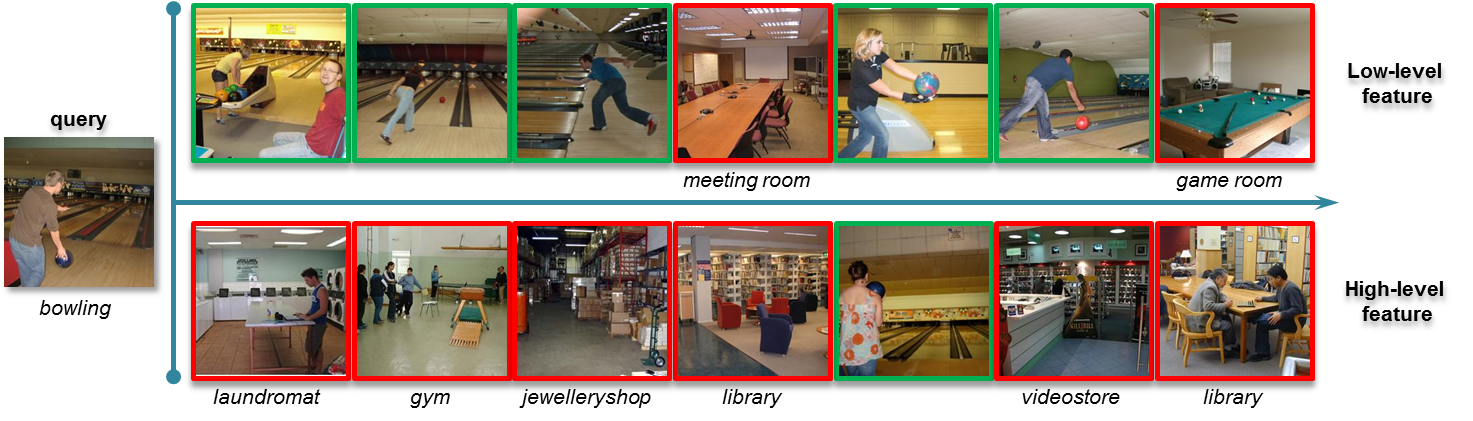
\includegraphics[width=.9\textwidth]{fig/moti_low_better.png}\label{fig:moti_low}}
	\subfigure[high-level feature is preferred]{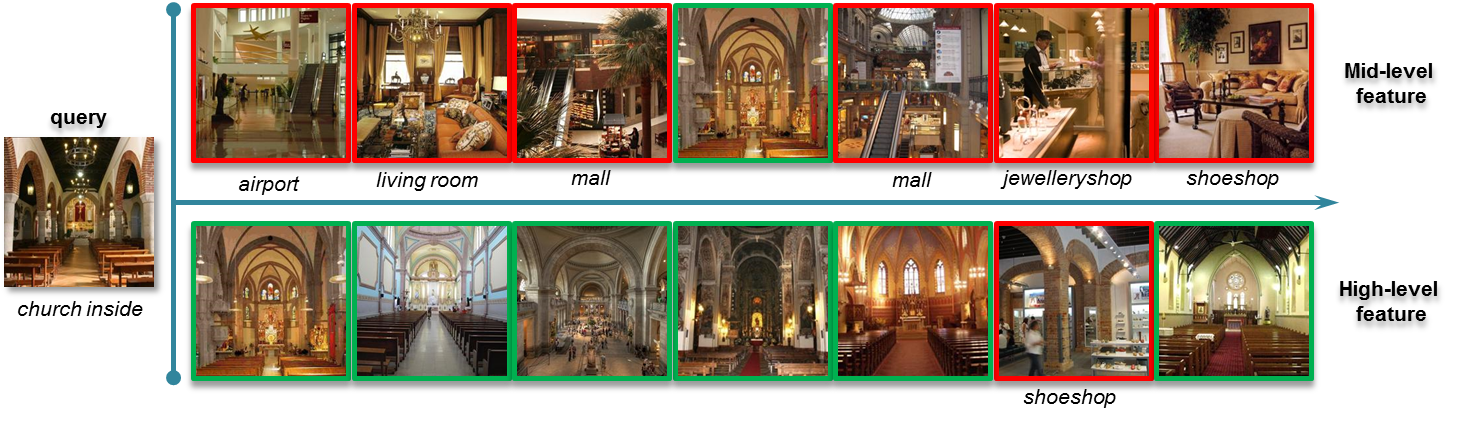
\includegraphics[width=.9\textwidth]{fig/moti_high_better.png}\label{fig:moti_high}}

\caption{Retrieval results using L2 distance for both mid- and high-level features on MIT67~\cite{MIT67}, computed from layer 11 and 20 of the Caffe model. \textit{Green} (\textit{Red}) box means correct (wrong) results, in terms of the scene category label. The correct label for wrong retrievals are provided. The retrieval results are displayed such that the left-most image has the closest distance to the query, and vice versa. Certain query images (or categories) produce better matches with high-level features, while others produce better results with mid-level features. This motivates our multi-scale approach.}
\label{fig:moti}
\end{figure*}


{\bf Multi-scale features:} We introduce multi-scale CNN architectures that use features at multiple scales for output prediction (Fig.~\ref{fig:splash}). From one perspective, our architectures are quite simple. Typical approaches train a output predictor (e.g., a linear SVM) using features extracted from a single output layer. Instead, one can train an output predictor using features extracted from multiple layers. Note that these features come ``for free''; they are already computed in a standard feed-forward pass. 

{\bf Spatial pooling:} One difficulty with multi-scale approaches is feature dimensionality - the total number of features across all layers can easily reach hundred of thousands. This makes training even linear models difficult and prone to over-fitting. Instead, we use marginal activations computed from sum (or max) pooling across all spatial locations in a given activation layer. From this perspective, our models are similar to those that compute multi-scale features with spatial pooling, including multi-scale templates~\cite{felzenszwalb2008discriminatively}, orderless models\cite{Gong14}, spatial pyramids~\cite{spatial_pyramid}, and bag-of-words~\cite{sivic2003video}. Our approach is most related to \cite{Gong14}, who also use spatially pooled CNN features for scene classification. They do so by pooling together multiple CNN descriptors (re)computed on various-sized patches within an image. Instead, we perform a single CNN encoding of the entire image, extracting multiscale features ``for free''.

{\bf End-to-end training:} Our multi-scale model differs from such past work in another notable aspect. Our entire model is still a feed-forward CNN that is no longer chain-structured, but a directed-acyclic graph (DAG). DAG-structured CNNs can still be discriminatively trained in an end-to-end fashion, allowing us to directly learn multi-scale representations. %Multi-scale learning addresses one well-known difficulty of CNNs - the ``vanishing gradient'' problem~\cite{bengio1994learning}. During gradient-based learning, the gradient signal becomes progressively diluted as one back-propagates it through multiple layers, such that the bottom-most layer receives essentially no updates. Our multi-scale DAG structure connects all activation layers directly to the output, ensuring they all receive a strong gradient signal during learning.  
DAG structures are relatively straightforward to implement given the flexibility of many deep learning toolboxes~\cite{vedaldimatconvnet,Caffe,overfeat}. Our primary contribution is the demonstration that structures can capture multiscale features, which in turn allow for transfer learning between coarse and fine-grained classification tasks.

%yeilding state-of-the-art recognition results across various recognition benchmarks. 

% Trained with large number of instances, (such as ImageNet~\cite{ImageNet}), CNN is also an excel candidate for off-the-shelf feature extractions, results in outstanding performance in various recognition tasks~\cite{cnn_baseline}. In the meantime, a considerable amount of effort is spent on how to further improve the performance of CNN. On one hand, many are focus on techniques to efficiently and effective train a CNN. A good initialization need to be carefully selected~\cite{diff_cnn} in the beginning. Data augmentation~\cite{AlexNet} is recommended to improve the model performance as well. Drop-out~\cite{dropout} and momentum~\cite{momentum} are also necessary to prevent over-fitting and obtain superior models. On the other hand, different model components and architectures are proposed. Rectified linear units (ReLU)~\cite{AlexNet} add non-linearity and enrich the model complexity. Different pooling method, such as Distance Transform Pooling~\cite{dist_trans}, is adopted in~\cite{dpm_is_cnn}, allowing local deformations, as in the widely-used deformable part-based model (DPM)~\cite{dpm}. \cite{veryDeep} adopts a small $3\times 3$ receptive field to deepen the model, while maintaining less parameters. A network in network~\cite{nin} is proposed to enhance model discriminability for local patches within the receptive field. The award winning GoogLeNet~\cite{GoogLeNet} uses an \textit{Inception} model that is based on the Hebbian principle~\cite{Hebb}, \ie, neurons that fire together, wire together, the theoretical proof of which is provided by~\cite{dnn_proof} under constraints. 

%One question to ponder: is there any model-independent potential that is yet to be discovered. Although allowing local deformation, CNN encodes the the spatial information of multi-scale features. Conversely, by ignoring the spatial location of features, bag-of-feature like techniques~\cite{spatial_pyramid} achieves transformation invariance to some extend. As pointed out in~\cite{Gong14}, combining both type of features results in a better representation for recognition tasks with large variations, such as Scene classification~\cite{SUN397,MIT67}. Traditionally, when CNN is used for feature extraction, the activation of the first fully-connected (FC) layer is usually considered as the feature~\cite{overfeat, Gong14}. Using an off-the-shelf deep CNN model,~\cite{Gong14} explicitly extracts image patches from three scales and computes the feed-forward CNN activations for each patch for feature extraction. This algorithm is cumbersome due to the computation of multiple patches for one image. Besides, it can only encode the multi-scale features to a certain extend limited by the burden of the post processing, \ie, K-means and Principle Component Analysis (PCA). As a matter of fact, CNN feature is meant to encode multi-scale feature at each convolutional (Conv.) layer. Therefore, there is no need to extract multi-scale patches and only one feed-forward computation is sufficient to capture the activations of multi-scale features for one input image. 


%In this paper, we first conducted an empirical analysis on the feature discriminativeness of every unit of CNN model. By average-pooling at each layer, the output ignores global spatial information and results in a bag-of-feature representation. The bag-of-feature from ReLU is then found to carry the most performance gain at each layer. We have also observed a synergy of multi-scale activations results in a better discriminative representation. These observations tie closely to the vanishing gradient~\cite{diff_cnn} issue in the deep CNN literature. During the training of a CNN, the top layer can be easily saturated. The gradients in the back-propagation algorithm will not effective reach the lower levels, resulting in a model that focuses more high-level features. Thus, we proposed a model augmentation schema, BoMSA, that chains the ReLU at each layer to the ultimate loss function. This augmentation approach is not confined by model variations and can be applied to existing pre-trained models or re-training the model from the ground up. By explicitly linking the lower layers to the decision layer, we gear the training towards the bag-of-activations from all layers. Thus, the augmented model is designed to be robust to spatial translations while maintaining its discriminative power in the multi-scale fashion.

{\bf DAG Neural Networks:} DAG-structured neural nets were explored earlier in the context of recurrent neural nets \cite{baldi2003principled,graves2009offline}. Recurrent neural nets use feedback to capture dynamic states, and so typically cannot be processed with feed-forward computations. Previous work has also shown that long-range connections between neural layers can eliminate the vanishing gradient problem, but this is done in the context of memory-based networks~\cite{hochreiter1997long}. We make use of DAG structures to efficiently encode multi-scale features in a simpler feed-forward network. 

{\bf Skip connections:} Our DAG structures are similar to recent networks that make use of ``skip'' connections between layers \cite{raiko-aistats-12,szegedy2014going,sermanet2013pedestrian}. \cite{raiko-aistats-12} show that such connections are useful for a single binary classification task, but we motivate multiscale connections through multitask learning: different visual classification tasks require features at different image scales. %Indeed, we show that off-the-shelf multi-scale features transfer extraordinary well between classification tasks. 
Finally, the recent state-of-the-art model of \cite{szegedy2014going} make use of skip connections for training, but does not use them at test-time. This means that the final feedforward predictor is not a DAG, though our results suggest that adding multiscale connections at testtime might further improve performence.
%multiscale features at test-time might further improve their performance.

{\bf Overview:} We motivate our multi-scale DAG-CNN model in Sec.~\ref{sec:motivation}, describe the full architecture in Sec.~\ref{sec:approach}, and conclude with numerous benchmark results in Sec.~\ref{sec:exp}. We evaluate multi-scale DAG-structured variants of existing CNN architectures (\eg, Caffe~\cite{Caffe}, Deep19~\cite{veryDeep}) on a variety of scene recognition benchmarks including SUN397~\cite{SUN397}, MIT67~\cite{MIT67}, Scene15~\cite{Scene15}. We observe a consistent improvement regardless of the underlying CNN architecture, producing state-of-the-art results on all 3 datasets.

%A consistent performance improvement is observed of our multi-scale representation over the best discriminative single-scale feature. 
%The rest of the paper is organized as follows: we motivate and describe our model augmentation approach in Sec.~
%\ref{sec:approach}. An in-depth analysis is provided in Sec.~\ref{sec:ana}. Systematic experimental results are included in Sec.~\ref{sec:exp}. 


%-------------------------------------------------------------------------
%-------------------------------------------------------------------------
\section{Motivation\label{sec:motivation}}

In this section, we motivate our multi-scale architecture with a series of empirical analysis. We carry out an analysis on existing CNN architectures, namely Caffe and Deep19. Caffe~\cite{Caffe} is a broadly used CNN toolbox. It includes a pre-trained model ``AlexNet''~\cite{AlexNet} model, learned with millions of images from the ImageNet dataset~\cite{ImageNet}. This model has 6 conv. layers and 2 fully-connected (FC) layers. Deep19~\cite{veryDeep} uses very small $3\times 3$ receptive fields, but an increased number of layers -- 19 layers (16 conv. and 3 FC layers). This model produced state-of-the-art performance in ILSVRC-2014 classification challenge~\cite{ILSVRC14}. We evaluate both ``off-the-shelf'' pre-trained models on the heavily benchmarked MIT Indoor Scene (MIT67) dataset~\cite{MIT67}, using 10-fold cross-validation.

\subsection{Single-scale models} 
%We first verify our hypothesis that different recognition tasks require different amounts of invariance through two experiments.

{\bf Image retrieval:} Recent work that explores sparse reconstruction techniques for visualizing and analyzing features~\cite{vondrick2013hoggles}. Inspired by such techniques, we use image retrieval to begin our exploration. We attempt to ``reconstruct'' a query image by finding $M=7$ closest images in terms of L2-distance, when computed with mean-pooled layer-specific activations. Results are shown for two query images and two Caffe layers in Fig.~\ref{fig:moti}. The {\tt florist} query image tends to produces better matches when using mid-level features that appear to capture \textit{objects} and \textit{parts}. On the other hand, the {\tt church-inside} query image tends to produce better matches when using high-level features that appear to capture more global \textit{scene} statistics.


%By working with poo providing some degree of robustness to spatial transformation of objects (bowling ball and people body parts). On the other hand, the example in Fig.~\ref{fig:moti_high} shows high-level feature captures the spatial geometry information. This is important for classes such as scenes with strong \textit{structure} cues, \eg, church, cloister, corridor, etc. Thus, we wish to develop a method that captures the multi-scale invariance.



%\subsection{Scale-specific classification}
%We carry out an analysis on existing CNN architectures, namely Caffe and Deep19. Caffe~\cite{Caffe} is a broadly used CNN toolbox. It includes a pre-trained model ``AlexNet''~\cite{AlexNet} model, learned with millions of images from the ImageNet dataset~\cite{ImageNet}. This model has 6 conv. layers and 2 fully-connected (FC) layers. Deep19~\cite{veryDeep} uses very small $3\times 3$ receptive fields, but an increased number of layers -- 19 layers (16 conv. and 3 FC layers). This model produced state-of-the-art performance in ILSVRC-2014 classification challenge~\cite{ILSVRC14}. We evaluate both models on the heavily benchmarked MIT Indoor Scene (MIT67) dataset~\cite{MIT67}.

\begin{figure}[t!]
\centering
	\subfigure[Caffe]{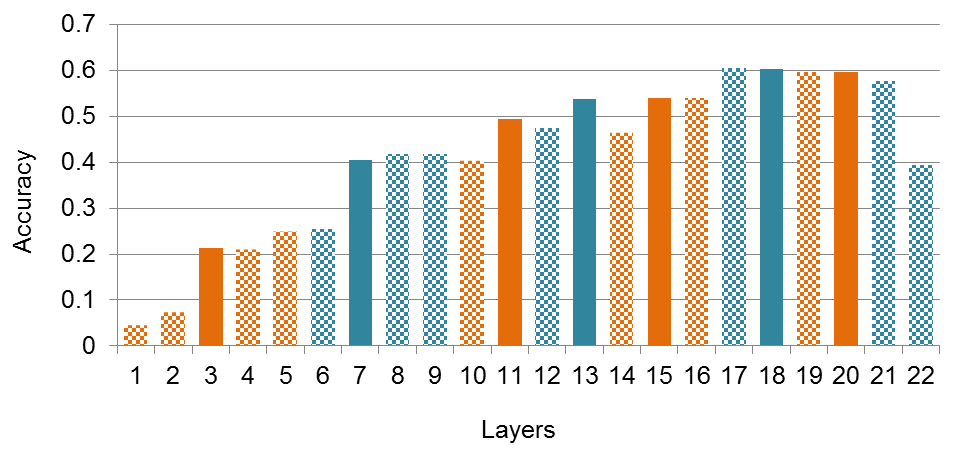
\includegraphics[width=\columnwidth]{fig/fig_layer_caffe.png}\label{fig:layer_caffe}}
	\subfigure[Deep19]{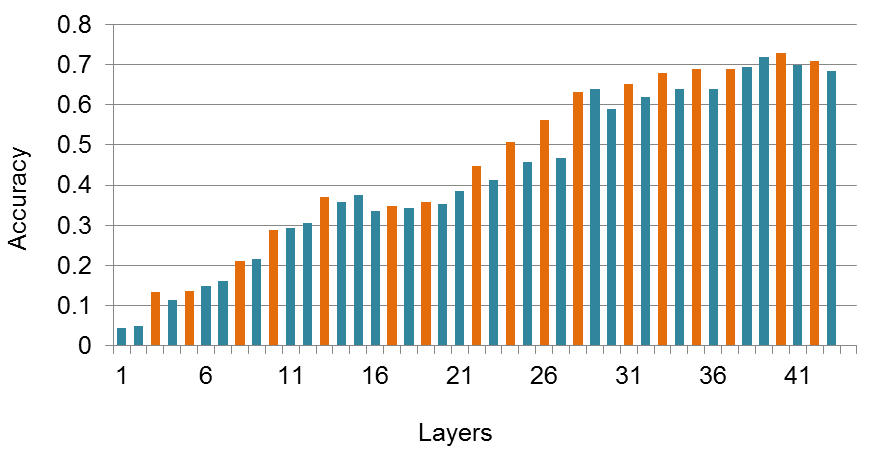
\includegraphics[width=\columnwidth]{fig/fig_layer_deep19.png}\label{fig:layer_deep19}}
\caption{The classification accuracy on MIT67~\cite{MIT67} using activations from each layer. We use a solid color fill representing the output of a ReLU layer. There are 7 ReLU layers for the Caffe model and 18 for Deep19. We see tend to see a performance jump at each successive ReLU layer, particularly earlier on in the model.}
\label{fig:layer_MIT67}
\end{figure}

{\bf Single-scale classification:} Following past work \cite{cnn_baseline}, we train a linear SVM classifier using features extracted from a particular layer. We specifically train $K=67$ 1-vs-all linear classifiers.
We plot the performance of single-layer classifiers in~\ref{fig:layer_MIT67}. The detailed parameter options for both Caffe and Deep19 models are described later in Sec.~\ref{sec:exp}. As past work has pointed out, we see a general increase in performance as we use higher-level (more invariant) features. We do see a slight improvement at each nonlinear activation (ReLU) layer. This makes sense as this layer introduces a nonlinear rectification operation $\max(0,x)$, while other layers (such an convolutional or sum-pooling) are linear operations that can be learned by a linear predictor.



\begin{figure*}[ht!]
\centering
	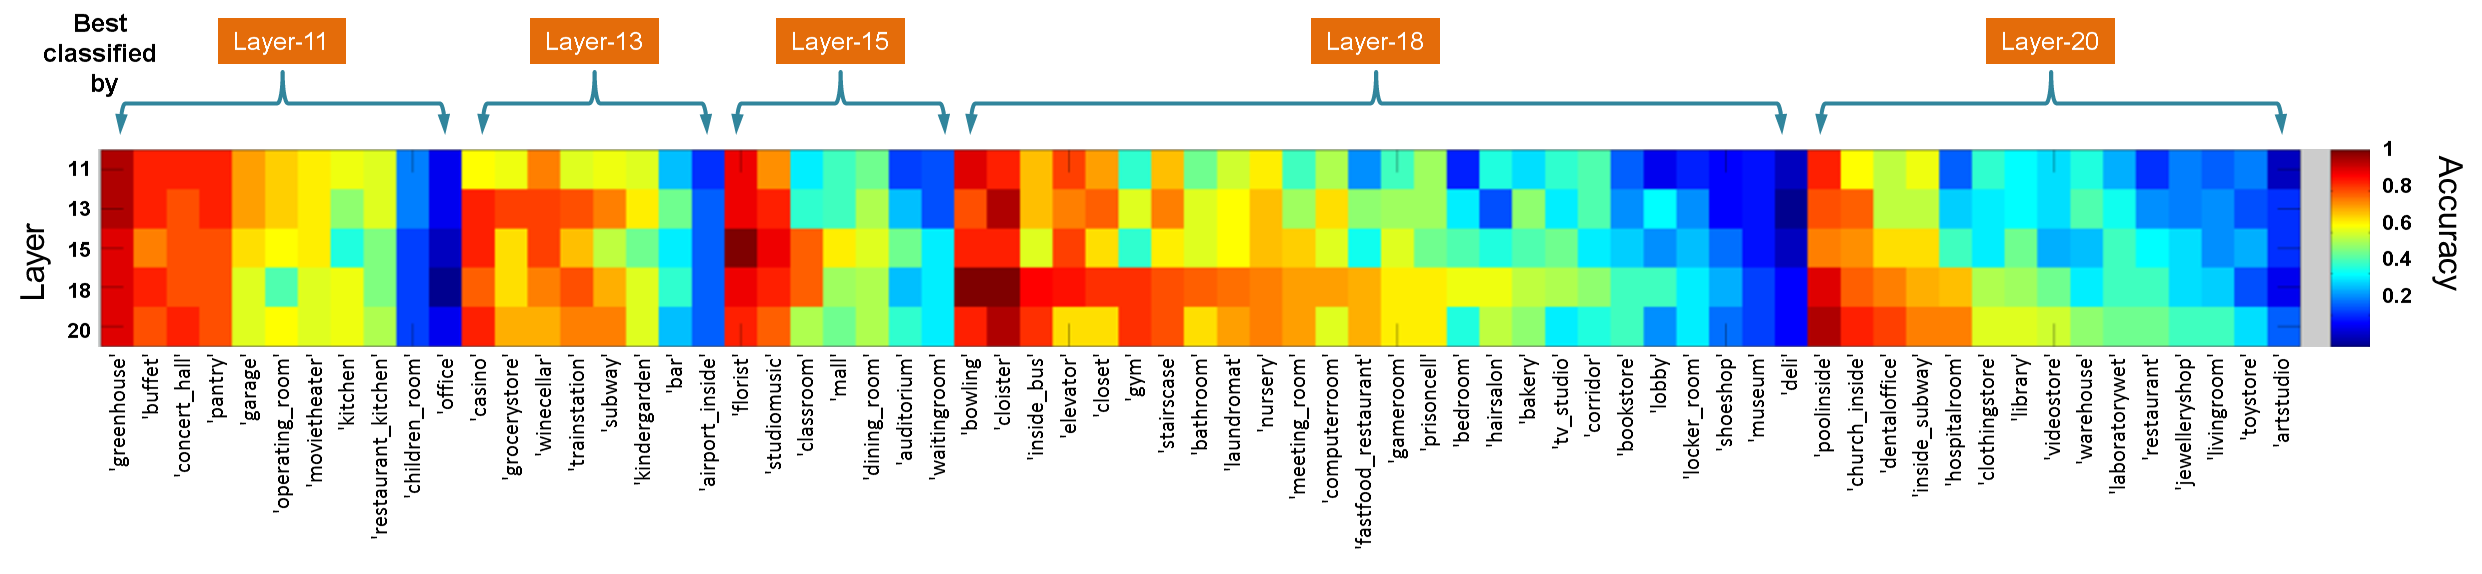
\includegraphics[width=1\textwidth]{fig/fig_level_perf.png}
\caption{The ``per-class'' performance using features extracted from particular layers. Certain groups of classes perform best using higher  or lower-level layers, each encoding different amounts of invariance. We further analyze this phenomena in Fig.~\ref{fig:best_perf_layer_hist}.}
\label{fig:level_perf}
\end{figure*}

\begin{figure}[t!]
\centering
	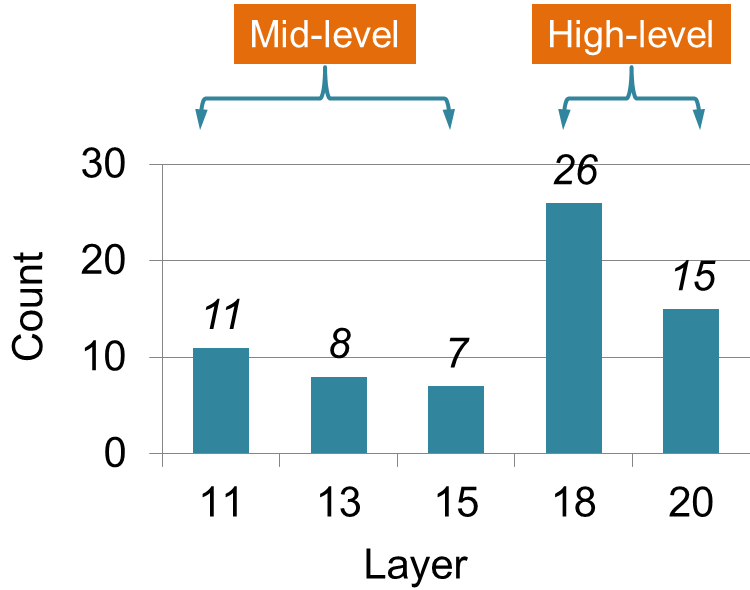
\includegraphics[width=.6\columnwidth]{fig/best_perf_layer_hist.png}
\caption{We count the number of classes with a particular best-performing layer. The last layer ({\bf 20}) is optimal for only 15 classes, while the second-to-last layer ({\bf 18}) proves most discriminative for 26 classes. The third-most effective layer ({\bf 11}) captures significantly lower-level level features. These results validate our underlying hypothesis; different classes require different amounts of invariance. This suggests that a feature extractor shared across such classes will be more effective when multi-scale.}
% A high-level feature (Layer-18) achieves the highest accuracy in the 26 categories. In the meantime, mid-level features (Layer-11,13, and 15) are also important in this classification task. They perform the best for another 26 categories. }
\label{fig:best_perf_layer_hist}
\end{figure}

{\bf Scale-varying classification:} The above experiment required training $K \times N$ 1-vs-all classifiers, where $K$ is the number of classes and $N$ is the number of layers. We can treat each of the $KN$ classifiers as binary predictors, and score each with the number of correct detections of its target class. We plot these scores as a matrix in Fig.~\ref{fig:level_perf}. We tend to see groups of classes that operate best with features computed from particular high-level or mid-level layers. Indeed, we plot the optimal scale for each binary predictor in Fig.~\ref{fig:best_perf_layer_hist}. Most categories tend to do well with high-level features, but a significant fraction (over a third) do better with mid-level features.

{\bf Spatial pooling:} In the next section, we will explore multi-scale features. One practical hurdle to including all features from all layers is the massive increase in dimensionality. Here, we explore strategies for reducing dimensionality through pooled features. We consider various pooling (sum, average, and max) and  normalization (with and without L2 normalization) strategies. We saw good results with average pooling over all spatial locations, followed by L2 normalization. Specifically, assume a particular layer is of size $H \times W \times F$, where $H$ is the height, $W$ is the width, and $F$ is the number of filter channels. We compute a $1 \times 1 \times F$ feature by averaging across spatial dimensions. We then normalize this feature to have unit norm. %Note that the ``marginal activations'' of fully-connected layers (which are already of dimension $1 \times 1 \times F$) are simply the original activations.  
We compare this encoding versus the full-dimensional feature (also normalized) in Fig.~\ref{fig:full_marg}. Pooled features always do better, implying dimensionality reduction actually helps performance. We verified that this phenomena was due to over-fitting; the full features always performed better on training data, but performed worse on test data. This suggests that with additional training data, less-aggressive pooling (that preserves some spatial information) may perform better. \deva{If we have time, we should explore other amounts of pooling; say pooling into quadrants such that the features is $2 \times 2 \times F$. One reviewer suggested this. This should be relatively easy to try out for single-scale. If it helps, we could try out for multi-scale and DAG.}

%{\bf Marginal vs full:} A reasonable question is whether some performance is sacrificed for this reduced dimensionality. To evaluate this hypothesis, we train an SVM on activations from a single layer, using both the full and marginal activations. For simplicity, we focus on the 5 best-performing layers from Fig.~\ref{fig:best_perf_layer_hist}. Surprisingly, the results in Fig.~\ref{fig:full_marg} shows that marginal features always outperform the full-dimensional feature, implying that dimensionality reduction actually helps performance. 
\begin{figure}[t!]
\centering
	{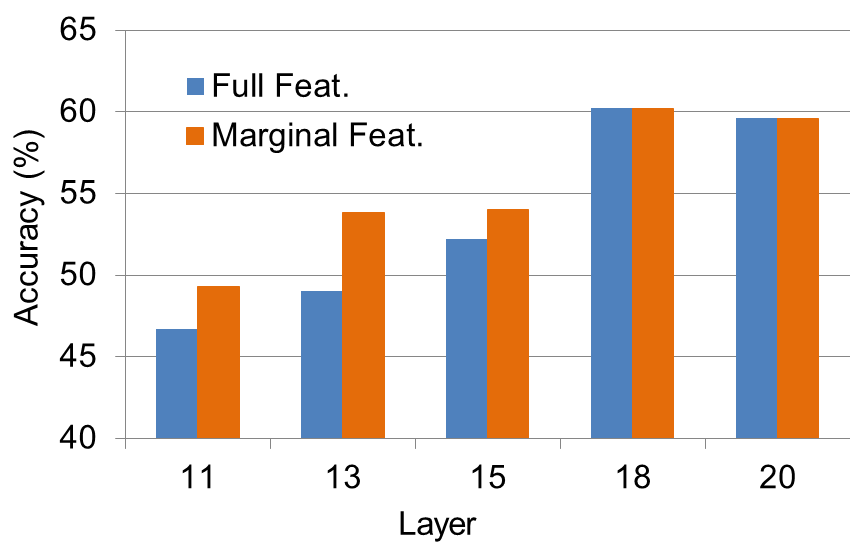
\includegraphics[width=.6\columnwidth]{fig/full_marg.png}}
\caption{Marginal features (computed by spatially-pooling across activations from a layer) do as well or better than their full-dimensional counterpart. }
\label{fig:full_marg}
\end{figure}


\subsection{Multi-scale models} 

{\bf Multiscale classification:} We now explore multi-scale predictors that process (marginal) features extracted from multiple layers. As before, we analyze ``off-the-shelf'' pre-trained models. We evaluate performance as we iteratively add more layers. Fig.~\ref{fig:layer_MIT67} suggests that the last ReLU layer is a good starting point due to its strong single-scale performance. Fig~\ref{fig:add_back} plots performance as we add previous layers to the classifier feature set. Performance increases as we add intermediate layers, while lower layers prove less helpful (and may even hurt performance, likely do to over-fitting). Our observations suggest that high and mid-level features (\ie, \textit{parts} and \textit{objects}) are more useful than low-features based on \textit{edges} or \textit{textures} in scene classification. 


% the performance increase in the beginning by adding mid-level features to enrich the model discriminativeness. However, including some low level responses to the feature actually hurts the performance, \ie, layer 7 and 3 in Fig.~\ref{fig:add_back_caffe}. 

%Since different CNN layers correspond to image feature at various scales, seen in Fig.~\ref{fig:moti}, we wonder whether combining activations at multiple scales help to extract a better feature. To address this question, we carried out another experiments on the MIT67 data~\cite{MIT67}. We start from the average-pooled response of the last ReLU layer and greedily concatenate the ones from previous ReLU layers. The reason we start from the last ReLU layer is that, in the literature when CNN is used for feature extraction, the response of the first fully connected layer is usually selected~\cite{cnn_baseline,Gong14}. Besides, our previous analysis in Fig.~\ref{fig:layer_MIT67} also demonstrates better discriminative power of high-level CNN layer.

%The rest of the experimental setups are the same as in Sec.~\ref{sec:indi_scale}, \ie, a set of 67-way one-vs-all linear SVM classifiers are trained every time we add one more layer. Since we keep on concatenating features at lower level, the feature dimension is monotonically increasing. As the results shown in Fig.~\ref{fig:add_back}, the performance increase in the beginning by adding mid-level features to enrich the model discriminativeness. However, including some low level responses to the feature actually hurts the performance, \ie, layer 7 and 3 in Fig.~\ref{fig:add_back_caffe}. We believe it demonstrates the benefit of incorporating more discriminative mid-level and high-level features of CNN (\ie, \textit{parts} and \textit{objects}), but not necessarily the low-level features, such as \textit{edge} or \textit{textures}. 

\begin{figure}[t!]
\centering
	\subfigure[Caffe]{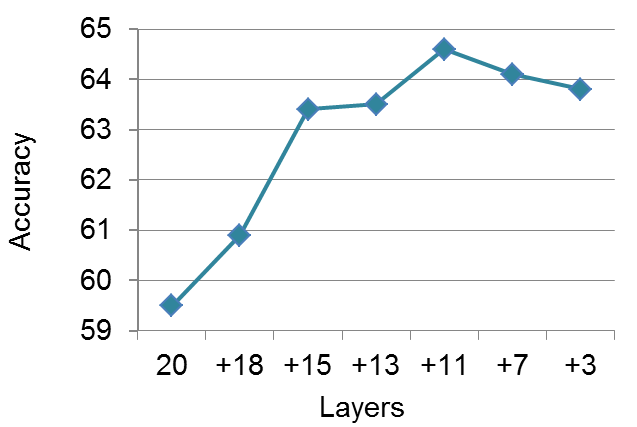
\includegraphics[width=.43\columnwidth]{fig/fig_add_back_caffe.png}\label{fig:add_back_caffe}}
	\subfigure[Deep19]{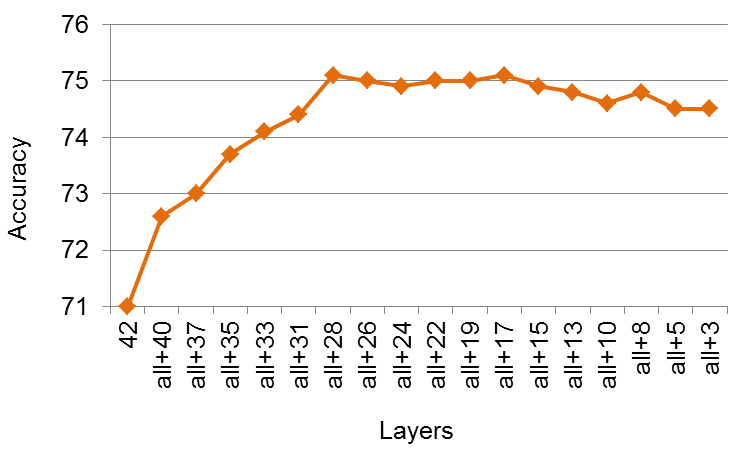
\includegraphics[width=.56\columnwidth]{fig/fig_add_back_deep19.png}\label{fig:add_back_deep19}}
\caption{We plot performance of a multi-scale classifier as we add more layer-specific features. We start with the last ReLU layer, and iteratively add the previous ReLU layer to the feature set of the classifier.
The ``+'' sign means the recent-most added layer. Adding additional layers help, but performance saturates and even slightly decreases when adding lower-layer features. This suggests it may be helpful to search for the ``optimal'' combination of layers.}
\label{fig:add_back}
\end{figure}

{\bf Multi-scale selection:} The previous results show that adding all layers may actually hurt performance. We verified that this was an over-fitting phenomena; additional layers always improved training performance, but could decrease test performance due to over-fitting. This appears especially true for multi-scale analysis, where nearby layers may encoded redundant or correlated information (that is susceptible to over-fitting). Ideally, we would like to search for the ``optimal'' combination of ReLU layers that maximize performance on validation data. Since there exists an exponential number of combinations ($2^N$ for $N$ ReLU layers), we find an approximate solution with a greedy forward-selection strategy. We greedily select the next-best layer (among all remaining layers) to add, until we observe no further performance improvement. As seen in Fig.~\ref{fig:forward_select_caffe}, the optimal results of this greedy approach rejects the low-level features. This is congruent with the previous results in Fig.~\ref{fig:add_back_caffe}. Similarly for the Deep19 model in Fig.~\ref{fig:forward_select_deep19}, although the feature pool is large (18 ReLU layers), the optimal greedy results includes only the mid- or high-level features. 

\begin{figure}[htbp]
\centering
	\subfigure[Caffe]{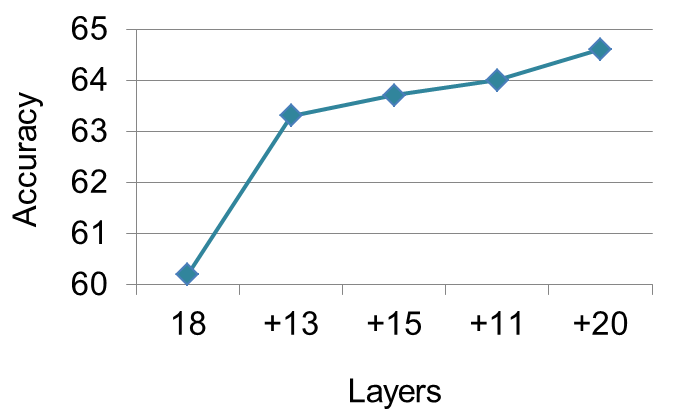
\includegraphics[width=.49\columnwidth]{fig/fig_forward_select_caffe.png}\label{fig:forward_select_caffe}}
	\subfigure[Deep19]{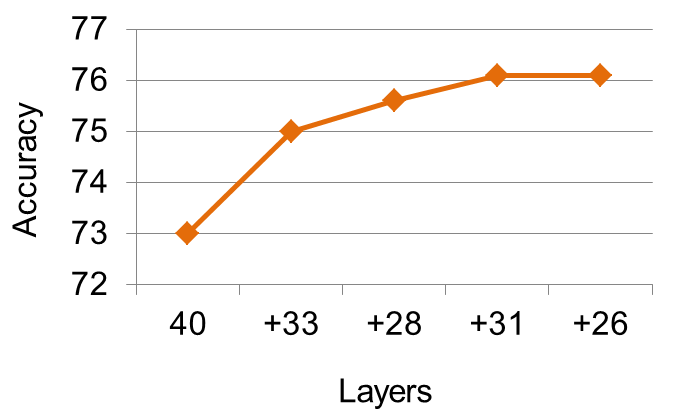
\includegraphics[width=.49\columnwidth]{fig/fig_forward_select_deep19.png}\label{fig:forward_select_deep19}}
\caption{The performance trend when using forward selection to incorporate the ReLU layers. Note that layers are {\em not} selected in high-to-low order. For example, both models begin with the second-to-last ReLU layer, and skip one or more previous layers when adding the next layer. This suggests that layers encode some redundant or correlated information. Overall, we see significant improvements of 3-5\% for both models.}% These results suggest that an ``off-the-shelf'' multi-scale model is already quite effective. We will show that ``fine-tuning'' with gradient-based DAG-CNN learning further improves results. Our performance increase comes with virtually no run-time cost, as these multi-scale features are already computed ``for free''.}
\label{fig:forward_select}
\end{figure}


Our analysis strongly suggest the importance (and ease) of incorporating multi-scale features for classification tasks. For our subsequent experiments, we use scales selected by the forward selection algorithm on MIT67 data (shown in Fig.~\ref{fig:forward_select}). Note that we use them for all our experimental benchmarks, demonstrating a degree of cross-dataset generalization in our approach.

\section{Approach\label{sec:approach}} 

In this section, we show that the multi-scale model examined in Fig.~\ref{fig:forward_select} can be written as a DAG-structured, feed-forward CNN. We also demonstrate that it can be trained with gradient-based learning. Essentially, one can use standard calculus constructions -- specifically the chain rule and partial derivatives -- to generalize back-propagation to layers that have multiple ``parents'' or inputs. Though such DAG structures have been previously introduced by prior work, we have not seen derivations for the corresponding gradient computations. We include them here for completeness, pointing out several opportunities for speedups given our particular structure.

{\bf Model:} The run-time behavior of our multi-scale predictor from the previous section is equivalent to feed-forward processing of the DAG-structured architecture in Fig.~\ref{fig:forward_select}. Note that we have swapped out a margin-based hinge-loss (corresponding to a SVM) with a softmax function, as the latter is more amenable to training with current toolboxes. Specifically, typical CNNs are grouped into collections of four layers, \ie, Conv., ReLU, contrast normalization (Norm), pooling layers (with the Norm and pooling layers being optional). The final layer is usually a $K$-way softmax function that predicts one of $K$ outputs. We visualize these layers as a chain-structured ``backbone'' in Fig.~\ref{fig:model}. Our DAG-CNN simply links each ReLU layer to an average-pooling layer, followed by a $L2$ normalization layer, which feeds to a fully-connected (FC) layer that produces $K$ outputs (represented formally as a $1 \times 1 \times K$ matrix). These outputs are element-wise added together across all layers, and the resulting $K$ numbers are fed into the final softmax function. The weights of the FC layers are equivalent to the weights of the final multi-scale $K$-way predictor (which is a softmax predictor for a softmax loss output, and a SVM for a hinge-loss output). Note that all the required operations are standard modules except for the \textit{Add}.

%modifications require standard layers, except for the \textid{Add}. Crucially, it breaks the chain-structure of the 


%Before connecting into the softmax layer, an \textit{Add} layer is introduced to combine the responses from all FC layers. 

\begin{figure*}[t!]
\centering
	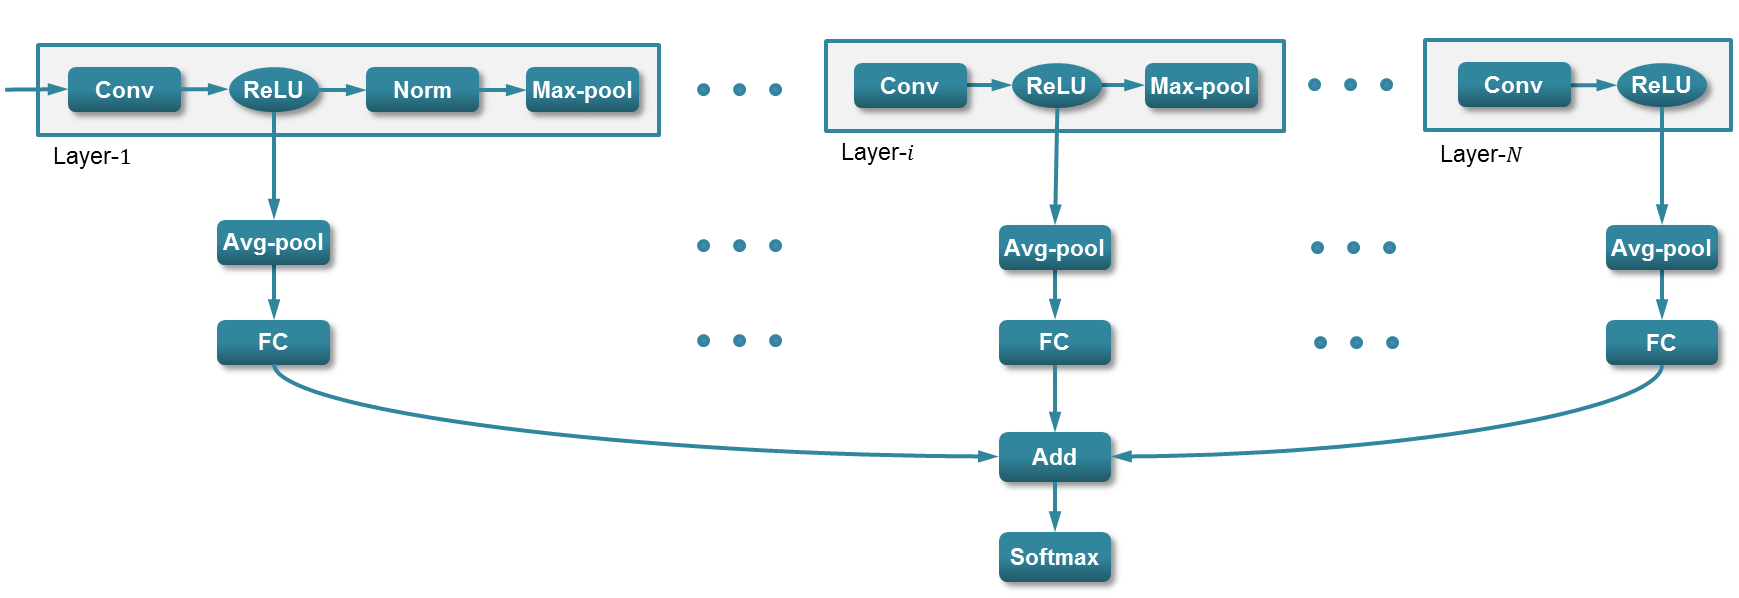
\includegraphics[width=\textwidth]{fig/fig_model.png}
\caption{Our multi-scale DAG-CNN architecture is constructed by adding multi-scale output connections to an underlying {\em chain backbone} from the original CNN. Specifically, for each scale, we spatially (average) pool activations, normalize them to have unit-norm, compute an inner product with a fully-connected (FC) layer with $K$ outputs, and add the scores across all layers to predictions for $K$ output classes (that are finally soft-maxed together).}
\label{fig:model}
\end{figure*}

{\bf Training:} Let $\textbf{w}_1,...\textbf{w}_K$ be the CNN model parameters at $1,..,K$-th layer, training data be ($\textbf{x}^{(i)},\textbf{y}^{(i)}$), where $\textbf{x}^{(i)}$ is the $i$-th input image and $\textbf{y}^{(i)}$ is the indicator vector of the class of $\textbf{x}^{(i)}$. Then we intend to solve the following optimization problem

\begin{align}
\argmin_{\textbf{w}_1,...\textbf{w}_K} \frac{1}{n}\sum_{i=1}^{n} \mathcal{L}(f(\textbf{x}^{(i)};\textbf{w}_1,...,\textbf{w}_K),\textbf{y}^{(i)})
\end{align}

As is now commonplace, we make use of stochastic gradient descent to minimize the objective function. For a traditional \textit{chain} model, the partial derivative of the output with respect to any one weight can be recursively computed by the chain rule, as described in the back-prop algorithm~\cite{rumelhart1988learning}. 

{\bf Multi-output layers (ReLU):} Our DAG-model is structurally different at the ReLU layers (since they have multiple outputs) and the \textit{Add} layer (since it has multiple inputs). We can still compute partial derivatives by recursively applying the chain rule, but care needs to be taken at these points. Let us consider the $i$-th ReLU layer in Fig.~\ref{fig:backprop_eq}. Let $\alpha_i$ be its input, $\beta_i^{(j)}$ be the output for its $j$-th output branch (its $j^{th}$ child in the DAG), and let $z$ is the final output of the softmax layer. The gradient of $z$ with respect to the input of the $i$-th ReLU layer can be computed as

\begin{align}
\frac{\partial z}{\partial \alpha_i}=\sum_{j=1}^{C}\frac{\partial z}{\partial \beta_i^{(j)}}\frac{\partial \beta_i^{(j)}}{\partial \alpha_i} \quad \text {(in general)} \label{eq:backprop1}
\end{align}

\noindent where $C=2$ for the example in Fig.~\ref{fig:backprop_eq}. One can recover standard back-propagation equations from the above by setting $C=1$: a single back-prop signal $\frac{\partial z}{\partial \beta_i^{(1)}}$  arrives at ReLU unit $i$, is multiplied by the local gradient $\frac{\partial \beta_i^{(1)}}{\partial \alpha_i^{(1)}}$, and is passed on down to the next layer below. In our DAG, {\em multiple} back-prop signals arrive $\frac{\partial z}{\partial \beta_i^{(j)}}$ from each branch $j$, each is multiplied by an branch-specific gradient $\frac{\partial \beta_i^{(j)}}{\partial \alpha_i}$, and their total sum is passed on down to the next layer.

% Each partial derivative component, $\frac{\partial z}{\partial \beta_i^{(j)}}\frac{\partial \beta_i^{(j)}}{\partial \alpha_i}$, can be computed in the typical back-prop fashion. In chain-structured back-propogration, a single back-prop signal \frac{\partial z}{\partial \beta_i} will arrive at ReLU unit $i$. This is multiped by the layer-specific gradient $
%This means that during gradient updating, multiple $(C)$ backprop signals will arrive at the $i^{th}$ ReLU layer. These signals are added together, and then 

\begin{figure}[htbp]
\centering
	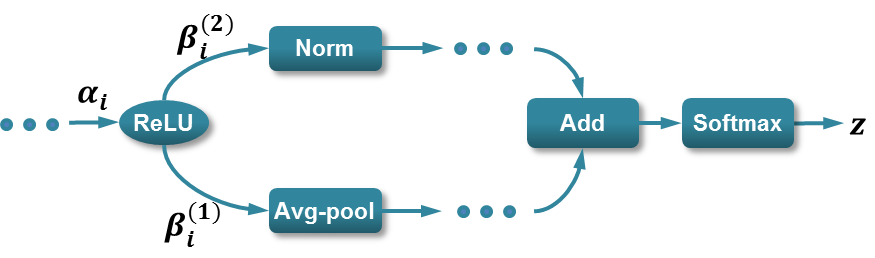
\includegraphics[width=\columnwidth]{fig/fig_backprop_eq.png}
\caption{Visualization of the parameter setup at $i$-th ReLU.}

\label{fig:backprop_eq}
\end{figure}

%Even though the Add layer is functionally quite simple, let us abstract its operation to a \textit{Combine} layer, $g(\cdot)$ that processes multiple inputs $\beta_k=g(\alpha^{(1)}_k,\cdots,\alpha^{(N)}_k)$ and $\alpha^{(j)}_k=h(\alpha_i)$. 
{\bf Multi-input layers (Add):} Let $\beta_k=g(\alpha^{(1)}_k,\cdots,\alpha^{(N)}_k)$ represents the output of a layer with multiple inputs. We can compute the gradient along the layer by applying the chain rule as follows:
\begin{align}
\frac{\partial z}{\partial \alpha_i}&=\frac{\partial z}{\partial \beta_k}\frac{\partial \beta_k}{\partial \alpha_i} \nonumber \\
&=\frac{\partial z}{\partial \beta_k}\sum_{j=1}^{C}\frac{\partial \beta_k}{\partial \alpha_k^{(j)}}\frac{\partial \alpha_k^{(j)}}{\partial \alpha_i} \quad \text{(in general)} \label{eq:backprop2}
\end{align} 
One can similarly arrive at the standard back-propagation by setting $C=1$.
% In chain-structured back-propogration, a single back-prop signal $\frac{\partial z}{\partial \beta_K}$ is arrives at the Add, is multipled by the local gradient 

 % arrives at ReLU unit $i$, is multipled by the local gradient $\frac{\beta_i}{\partial \alpha_i}$, and is passed on down to the next layer below. In our DAG, {\em multiple} backprop signals arrive $\frac{\partial z}{\partial \beta_i^{(j)}}$ from each branch $j$, each is multipled by an branch-specific gradient $\frac{\partial \beta_i^{(j)}}{\partial \alpha_i}$, and their total sum is passed on down to the next layer.


{\bf Special case (ReLU):} Our particular DAG architecture can further simplify the above equations. Firstly, it may be common for multiple-output layers to duplicate the same output for each child branch. This is true of our ReLU units; they pass the same values to the next layer in the chain and the current-layer pooling operation. This means the output-specific gradients are identical for those outputs $\forall j, \frac{\partial \beta_i^{(j)}}{\partial \alpha_i} =  \frac{\partial \beta_i^{(1)}}{\partial \alpha_i}$, which simplifies \eqref{eq:backprop1} to
\begin{align}
\frac{\partial z}{\partial \alpha_i} = \frac{\partial \beta_i^{(1)}}{\partial \alpha_i} \sum_{j=1}^{C}\frac{\partial z}{\partial \beta_i^{(j)}} \quad \text{(for duplicate outputs)}
\end{align}
This allows us to add together multiple back-prop signals before scaling them by the local gradient, reducing 
the number of multiplications by $C$. We make use of this speed up to train our ReLU layers
. 

{\bf Special case(Add):} Similarly, our multi-input {\tt Add} layer reuses the same partial gradient for each input
$\forall j, \frac{\partial \beta_k}{\partial \alpha_k^{(j)}} = \frac{\partial \beta_k}{\partial \alpha_k^{(1)}}$ which simplifies even further in our case to $1$. The resulting back-prop equations that simplify \eqref{eq:backprop2} are given by
\begin{align}
\frac{\partial z}{\partial \alpha_i} = \frac{\partial z}{\partial \beta_k} \frac{\partial \beta_k}{\partial \alpha_k^{(1)}}\sum_{j=1}^{C} \frac{\partial \alpha_k^{(j)}}{\partial \alpha_i}  \quad \text{(for duplicate gradients)}
\end{align}
\noindent implying that one can similarly save $C$ multiplications. The above equations have an intuitive implementation; the standard chain-structured back-propagation signal is simply replicated along each of the parents of the {\tt Add} layer.

{\bf Implementation:} We use the excellent MatConNet codebase to implement our modifications \cite{vedaldimatconvnet}. We implemented a custom {\tt Add} layer and a custom DAG data-structure to denote layer connectivity. Training and testing is essentially as fast as the chain model.

{\bf Vanishing gradients:} We point out an interesting property of our multiscale models that make them easier to train. Vanishing gradients~\cite{bengio1994learning} refers to the notorious poperty of deep models that make them difficult to train. Essentially, gradient magnitudes decrease as they are propogated, implying that lower-layers can be difficult to learn because they recieve too small a learning signal. In our DAG-CNNs, lower layers are directly connected to the output layer through multi-scale connections, ensuring they receive a strong gradient signal during learning. Fig.~\ref{fig:grad} experimentally verifies this claim.% DAG-CNN at the bottom layer is consistently larger than that of a chain model during training time. This make multi-scale training considerably more efficient than single (e.g., high-level) scale training.

\begin{figure}[htbp]
\centering
%Gradient-based learning\\
%\rotatebox{90}{\small \hspace{0pt} Average gradient \\(in log scale)}	
%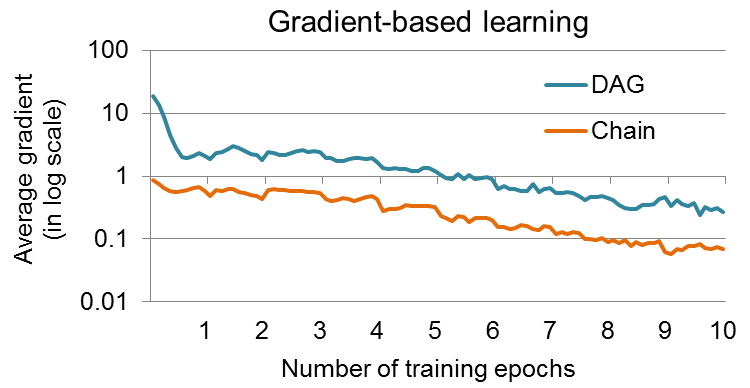
\includegraphics[width=.8\columnwidth,clip=true,trim=10mm 10mm 0mm 0mm]{fig/fig_grad.png}\\{\footnotesize Number of training epochs}
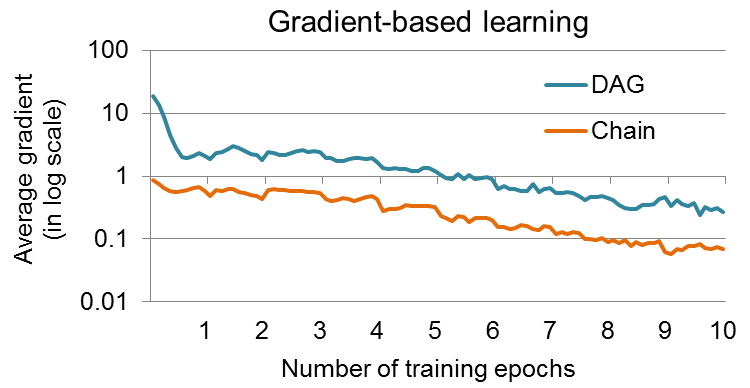
\includegraphics[width=.9\columnwidth]{fig/fig_grad.png}
\caption{The average gradient from Layer-1 (Conv.) during training, plotted in log-scale. Gradients from the DAG are consistently $10\times$ larger, implying that they receive a stronger supervised signal from the target label during gradient-based learning.}
\label{fig:grad}
\end{figure}


%{\bf Off-the-shelf DAG:} We point out an interesting instantiation of our model, linking back to the analysis in Section~\ref{sec:motivation}. We could switch the softmax loss to hinge loss and freeze the back-prop at the FC layers. In this way, we prevent altering the chaining backbone of the model, \ie, we learn an linear combination of the FC layers represents multi-scale ReLU activations. Thus, this is equivalent of training a SVM classifier based on the concatenation of the average-pooled activations at all ReLUs. As a result, we could extract multi-scale features using pre-trained CNN models such as the ones in~\cite{AlexNet, veryDeep} and use off-the-shelf SVM solver such as~\cite{liblinear} to train our DAG-CNN model. We compare to such an off-the-shelf DAG in our experiments, showing that they already produce state-of-the-art results.

%-------------------------------------------------------------------------
%-------------------------------------------------------------------------
\section{Experimental Results\label{sec:exp}}

In this section, we conduct experiments on benchmark datasets, SUN397~\cite{SUN397}, MIT67~\cite{MIT67}, and Scene15~\cite{Scene15}. In absolute terms, we have achieved the best performance ever reported on all three benchmarks. We also show more classification results in Fig.~\ref{fig:more_eg}. 

\subsection{Experiment Setup}
We stress that cross-validation on the MIT67 dataset is used to select the set of multi-scale layers in our DAG, as shown in Fig.~\ref{fig:forward_select}. The same set is then used for all other benchmark datasets. Our results may further improve through data-dependant scale selection. We explore DAG-structured variants of two popular models, Caffe~\cite{Caffe} and Deep19 models~\cite{veryDeep}. We follow the standard image pre-processing steps of fixing the input image size to $224\times 224$ by scaling and cropping, and subtracting out the mean RGB value (computed on ImageNet). 

{\bf Training:} We initialize filters and biases to their pre-trained values (tuned on ImageNet) and initialize multi-scale fully-connected (FC) weights to small normally-distributed numbers. We perform 10 epochs of learning.
%We follow the standard image pre-processing steps in the literature~\cite{AlexNet,Caffe,veryDeep}. Since both Caffe~\cite{Caffe} and Deep19 models~\cite{veryDeep} have a fixed input size of $224\times 224$, we first resize the image such that the smaller side matches $224$, and then crop an $224\times 224$ patch from the center. The mean RGB value of each model learned on ImageNet~\cite{ImageNet} is then subtracted.  

{\bf Feature dimensionality:} Most existing methods that use CNNs as feature extractors work with the last layer (or the last fully connected layer), yielding a feature vector of size 4096. Our multi-scale model generates a feature vector of size 9216, {\em making it only a factor of 2 larger} and so rather easy to use in practice. We provide the exact breakdown of feature dimensionality for our Caffe-DAG model in Table.~\ref{table:feat_dim}.
\begin{table}[t!]
\begin{center}
\begin{tabular}{|c|c|c|c|}
\hline
Layer & Response &  Full Feat.& Marginal Feat.\\
\hline
11 & $13\times 13 \times 384$ & 64896 & 384 \\
13 & $13\times 13 \times 384$ & 64896 & 384 \\
15 & $13\times 13 \times 256$ & 43264 & 256 \\
18 & $1\times 1 \times 4096$ & 4096 & 4096 \\
20 & $1\times 1 \times 4096$ & 4096 & 4096 \\
\hline
Total& & 181248 & 9216\\
\hline
\end{tabular}
\end{center}
\caption{Feature Dimension for Caffe-DAG. For reference, we also show the dimensionality obtained using all activations from a layer, rather than just the marginal ones. Marginal features reduce dimensionality by nearly 20X, while preserving accuracy (as shown in Fig.~\ref{fig:full_marg}).}
\label{table:feat_dim}
\end{table}

%\begin{table}[htbp]
%\begin{center}
%\begin{tabular}{|c|c|c|c|}
%\hline
%Layer & Response &  Full Feat.& Marg. Feat.\\
%\hline
%
%1 &	$227\times	227\times	3$ &	154587 &	3 \\
%2 &	$55\times	55\times	96$ &	290400 &	96 \\
%3 &	$55\times	55\times	96$ &	290400 &	96 \\
%4 &	$27\times	27\times	96$ &	69984 &	96 \\
%5 &	$27\times	27\times	96$ &	69984 &	96 \\
%6 &	$27\times	27\times	256$ &	186624 &	256 \\
%7 &	$27\times	27\times	256$ &	186624 &	256 \\
%8 &	$13\times	13\times	256$ &	43264 &	256 \\
%9	& $13\times	13\times	256$ &	43264 &	256 \\
%10 &	$13\times	13\times	384$ &	64896 &	384 \\
%11 &	$13\times	13\times	384$ &	64896 &	384 \\
%12 &	$13\times	13\times	384$ &	64896 &	384 \\
%13 &	$13\times	13\times	384$ &	64896 &	384 \\
%14 &	$13\times	13\times	256$ &	43264 &	256 \\
%15 &	$13\times	13\times	256$ &	43264 &	256 \\
%16 &	$6\times	6\times	256$ &	9216 &	256 \\
%
%\hline
%\end{tabular}
%\end{center}
%\caption{Full and Marginal feature dimension for Caffe-DAG}
%\label{table:feat_dim}
%\end{table} 


{\bf Baselines:} We compare our DAG models to published results, including two additional baselines. We evaluate the best single-scale ``off-the-shelf'' model, using both Caffe and Deep19. We pass L2-normalized single-scale features to Liblinear~\cite{liblinear} to train $K$-way one-vs-all classifiers with default settings. Finally, Sec.~\ref{sec:diag} concludes with a detailed diagnostic analysis comparing off-the-shelf and fine-tuned versions of chain and DAG structures.

%We show results of using our DAG-structure model for feature extraction. Thus, the output of all the average-pooled ReLU activations are concatenated as our multi-scale representation. For a fair comparison, we compare the multi-scale feature to the {\em best} performing single-scale feature. All features are $L2$-normalized before they are passed to the SVM solver. We use Liblinear~\cite{liblinear} to train $K$-way one-vs-all classifiers with default settings.


%-------------------------------------------------------------------------
\subsection{SUN397}

SUN397~\cite{SUN397} is a large scene recognition dataset with 397 categories, each of which includes more than 100 images. The total number of images exceeds 100k. The average classification accuracy is usually report from a 10-fold cross validation. The split file is provided in~\cite{SUN397} with 50 images for training and the rest being test for each fold.  


\begin{table}[htbp]
\begin{center}
\begin{tabular}{|l|c|}
\hline
Approach & Accuracy(\%) \\
\hline
Deep19-DAG & \textbf{56.2} \\
Deep19~\cite{veryDeep} & 51.9 \\
Caffe-DAG & 46.6	\\
Caffe~\cite{Caffe} & 43.5 \\ \hline
Places~\cite{zhoulearning}	& 54.3	\\
MOP-CNN~\cite{Gong14} & 52.0 \\
FV~\cite{FV} & 47.2 \\
DeCaf~\cite{DeCaf} & 40.9	\\
Baseline-overfeat~\cite{SUN_ijcv}	&40.3 \\
Baseline~\cite{SUN397} & 38.0 \\
\hline
\end{tabular}
\end{center}
\caption{Classification results on SUN397}
\label{table:SUN397}
\end{table}

We observe that features from our DAG-CNN feature always out-perform the single-scale feature for both DAG variants. In particular, Deep19-DAG achieves the highest $56.2\%$ accuracy. We should also point out that the next-best method of~\cite{zhoulearning} (with a score of $54.3$) makes use of a ImageNet-trained CNN and a custom-trained CNN using a new 7-million image dataset with 400 scene categories.
%, and makes use of  Places. Places contains over 7 million images in over 400 scene categories. Their performance of $54.3$ is achieved by the synergy of Place- and ImageNet-CNN features. 

%The authors of SUN397 database provided the baseline in the extended paper~cite{SUN_ijcv} using a set of traditional visual features, \eg, SIFT, GIST, etc. as well as the off-the-shelf deep CNN feature, Overfeat~\cite{overfeat}. The result is interesting such that Overfeat by itself ($40.3\%$) out-performs the combinations of all classical image features ($37.5\%$). 

%-------------------------------------------------------------------------
\subsection{MIT67}

MIT67 refers to the MIT Indoor~\cite{MIT67} scene classification for 67 categories. Indoor scenes depends on highly variable features to describe them. There are cases that can be well characterized by high-level spatial geometry (\eg~{\tt church} and {\tt cloister}) and mid-level objects (\eg~{\tt wine celler} and {\tt operating room}). The training/test split is made available and there are 80/20 training/test images for each class.

\begin{table}[htbp]
\begin{center}
\begin{tabular}{|l|c|}
\hline
Approach & Accuracy(\%) \\
\hline
Deep19-DAG & \textbf{77.5} \\
Deep19~\cite{veryDeep} & 70.8 \\
Caffe-DAG & 64.6	\\
Caffe~\cite{Caffe} & 59.5 \\ \hline
MOP-CNN~\cite{Gong14} & 68.9 \\
Places~\cite{zhoulearning}	& 68.2	\\
Mid-level~\cite{mid_level} & 64.0	\\
FV+BoP~\cite{FV_BoP} & 63.2 \\
Disc. Patch~\cite{disc_patch} & 49.4 \\
SPM~\cite{spatial_pyramid} & 34.4	\\
\hline
\end{tabular}
\end{center}
\caption{Classification results on MIT67}
\label{table:MIT67}
\end{table}

Our DAG-CNN model is designed to encode features across multiple scales and capture high- and mid-level statistics of scene categories. Similar observations can be drawn from Table.~\ref{table:MIT67}. The DAG-CNN models consistently out-perform the traditional chain model. The highest accuracy, $76.1\%$ is achieved by the DAG-CNN with Deep19 backbone. The method in~\cite{Gong14} also uses multi-scale features, and served as inspiration for our work. However, rather than extracting features from multiple layers of a CNN, they sample local patches at three different scales and resize each to a canonical scale that can be processed with an off-the-shelf CNN. Their method requires encoding large vocabularies through vector quantization, followed by multiple projection steps to keep feature dimension manageable. Our multi-scale representation, while similar in spirit, can be computed ``for free'' from a single (DAG) CNN.
% The activation of first fully connected layer is concatenated. Their method is less efficient to the the multiple runs of feed-forward computation and high dimensional features.


%-------------------------------------------------------------------------
\subsection{Scene15}

The Scene15~\cite{Scene15} includes both indoor scene (\eg, store and kitchen) and outdoor scene (\eg, mountain and street). A 10-fold split is provided with 1500 training and 2985 test image, where all images come in black and white. A consistent performance also is observed in Table.~\ref{table:Scene15}. 

\begin{table}[htbp]
\begin{center}
\begin{tabular}{|l|c|}
\hline
Approach & Accuracy(\%) \\
\hline
Deep19-DAG & \textbf{92.9} \\
Deep19~\cite{veryDeep} & 90.8 \\
Caffe-DAG & 89.7	\\
Caffe~\cite{Caffe} & 86.8 \\ \hline
Place~\cite{zhoulearning} & 91.6 \\
CENTRIST~\cite{Wu_pami11} & 84.8	\\
Hybrid~\cite{Bosch_pami08}	& 83.7	\\
Spatial pyramid~\cite{spatial_pyramid} & 81.4 \\
Object bank~\cite{Li_nips10_objectbank}	& 80.9	\\
Reconfigurable model~\cite{Parizi_cvpr12_reconf} & 78.6	\\
Spatial Envelop~\cite{Oliva_ijcv01_envelop} & 74.1 \\
Baseline~\cite{Scene15} & 65.2 \\
\hline
\end{tabular}
\end{center}
\caption{Classification results on Scene15}
\label{table:Scene15}
\end{table}


%-------------------------------------------------------------------------
%-------------------------------------------------------------------------
%\section{Discussion}

%In this section, we include additional details and diagnostic experiments on feature dimensionality, the effect of marginalization, and fine-tuning.

%\subsection{Feature dimension}

%{\bf Full vs. Marginal Features:} The above table suggests that it is crucial to use marginal features to keep the final dimensionality of the multi-scale feature manageable. A reasonable question is whether some performance is sacrificed for this reduced dimensionality. To evaluate this hypothesis, we build on the single-scale diagnostic experiments from our paper (Fig 3). Recall these experiments train and test an SVM on activations from a single-layer. We repeat these experiments using both full and marginal activation features each layer. For simplicity, we focus on 5 layers selected through forward selection (Fig.~\ref{fig:full_marg}).

%\begin{figure}[t!]
%\centering
%	{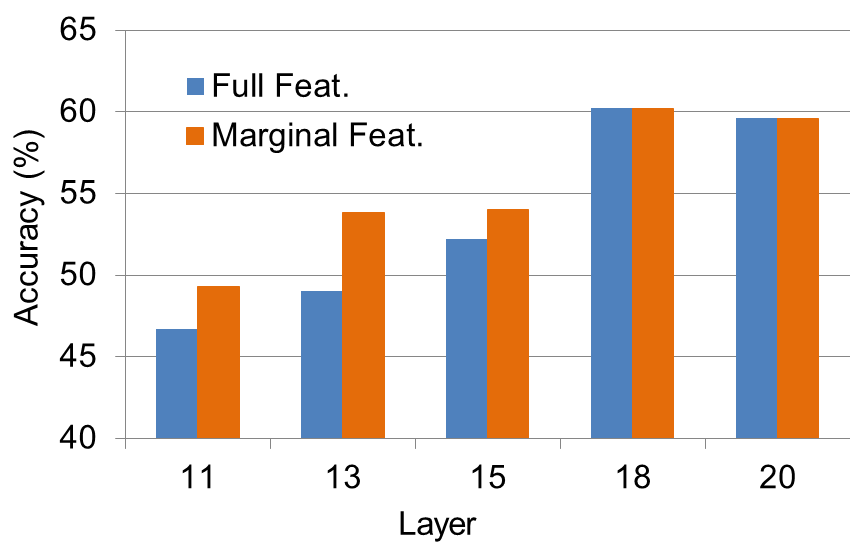
\includegraphics[width=.8\columnwidth]{fig/full_marg.png}}
%\caption{Single-scale classification accuracy (\%) of Full vs. Marginal Features.}
%\label{fig:full_marg}
%\end{figure}

%Surprisingly, we find that {\em marginal features always outperform the full dimensional feature}, implying that dimensionality reduction actually helps performance. We verified that this phenomena was due to over-fitting; the full features always performed better on training data, but performed worse on test data. This suggests that with additional training data, the full-dimensionality features may perform better.

\subsection{Diagnostics \label{sec:diag}}
In this section, we analyze ``off-the-shelf'' (OTS) and ``fine-tuned'' (FT) versions of both single-scale Chain and multi-scale DAG models. We focus on the Caffe model, as it is faster and easier for diagnostic analysis. 

{\bf Chain:} Chain-OTS uses single-scale features extracted from CNNs pre-trained on ImageNet. These are the baseline Caffe results presented in the previous subsections. Chain-FT trains a model on the target dataset, using the pre-trained model as an initialization. This can be done with standard software packages~\cite{vedaldimatconvnet}. To ensure consistency of analysis, in both cases features are passed to a K-way multi-class SVM to learn the final predictor. %We saw a small improvement in performance in doing this, rather than directly using the softmax prediction.

{\bf DAG:} Importantly, we explore an ``off-the-shelf'' version of our DAG, DAG-OTS.  Specifically, we fix all internal filters and biases to their pre-trained values, and only learn the fully-connected (FC) weights. This final stage learning is a convex problem, and can be done by simply passing the multi-scale features to a convex linear classification package (e.g., SVM). We compare this model to a fine-tuned version that is trained end-to-end, making use of the modified backprop equation from Sec.~\ref{sec:approach}. %We will show that off-the-shelf DAGs perform quite well, though fine-tuning does further improve performance.

{\bf Comparison:} Fig.~\ref{fig:comp_otf} reports the comparison of off-the-shelf and fine-tune features on both Chain and DAG models. Significant improvements of DAG over Chain are observed in all three datasets, suggesting that the multi-scale features indeed plays an essential role for scene classification. Further, fine-tuned features out-perform the off-the-shelf features consistently. This shows that the data specific information is well captured by fine-tuning, which further boosts the recognition performance. 

{\bf DAG-OTS:} Perhaps most impressive is the strong performance of DAG-OTS. From a theoretical perspective, this validates our underyling hypothesis that multi-scale features allow for better transfer between recognition tasks -- in this case, ImageNet and scene classification. An interesting question is whether multi-scale features, trained with our gradient-based DAG-learning on ImageNet, will allow for even more transfer. We are currently exploring this. However even with current CNN architectures, our results suggest that {\em any system making use of off-the-shelf CNN features should explore multi-scale variants as a ``cheap" and ``easy-to-implement'' baseline.}  Multiscale features require essentially no additional time to compute (compared to their single-scale counterparts),  are only a factor of 2 larger to store, and consistently provide a noticeable improvement.

%\begin{figure}[htbp]
%\centering
%	{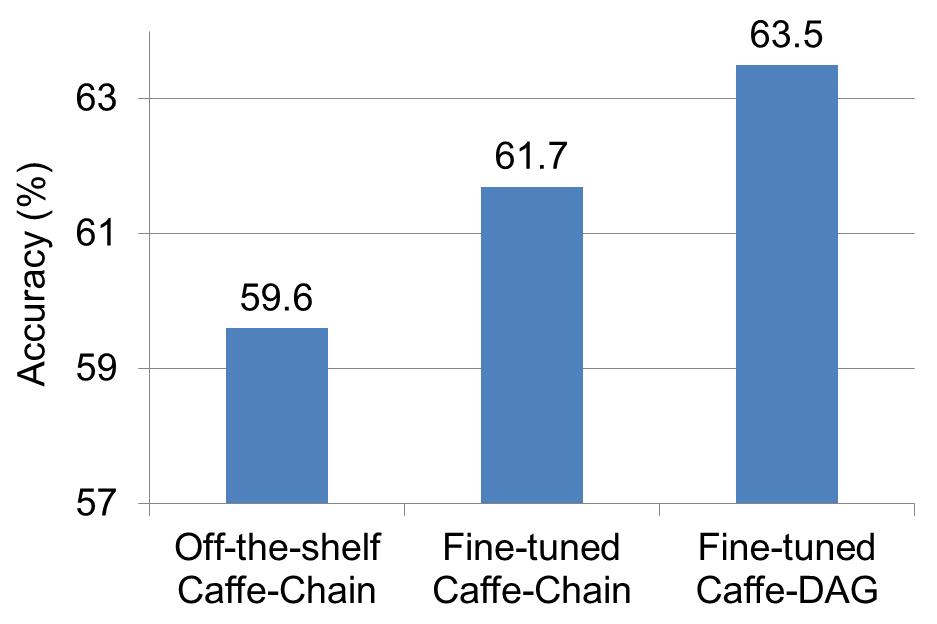
\includegraphics[width=.75\columnwidth]{fig/ft_model.png}}

%\caption{The comparison of fine-tune Models on MIT67.}
%\label{fig:ft_model}
%\end{figure}

%\begin{figure}[t]
%\centering
%	\subfigure[Chain]{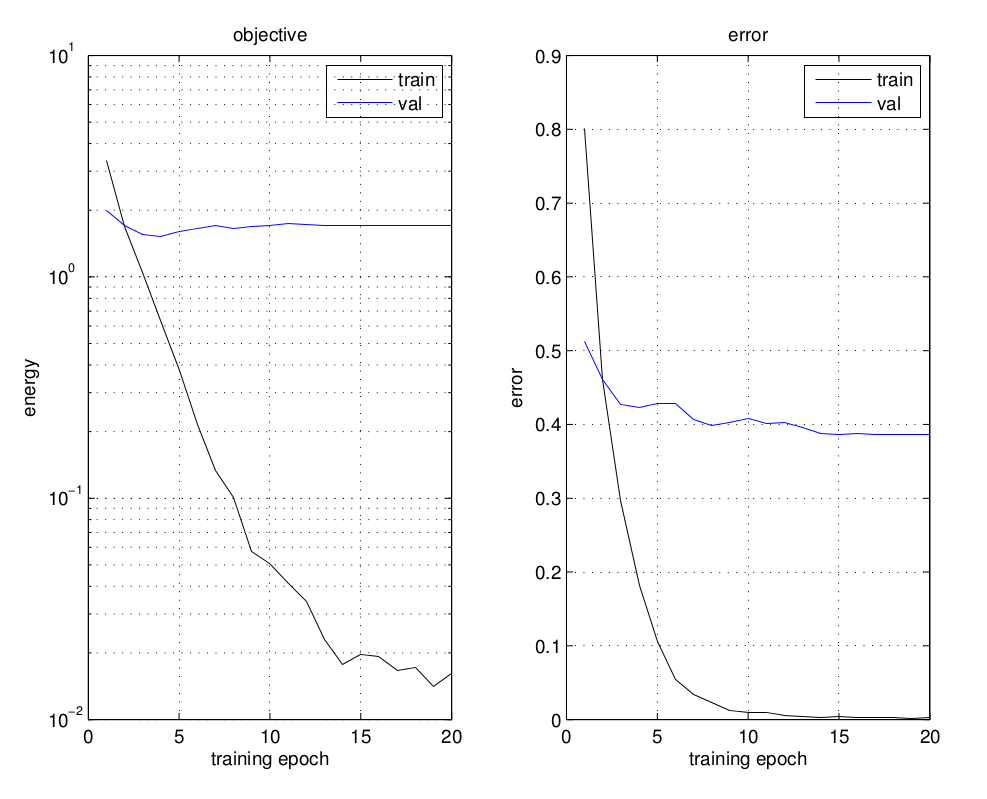
\includegraphics[width=.9\columnwidth]{fig/ft_chain.png}\label{fig:ft_chain}}
%	\subfigure[DAG]{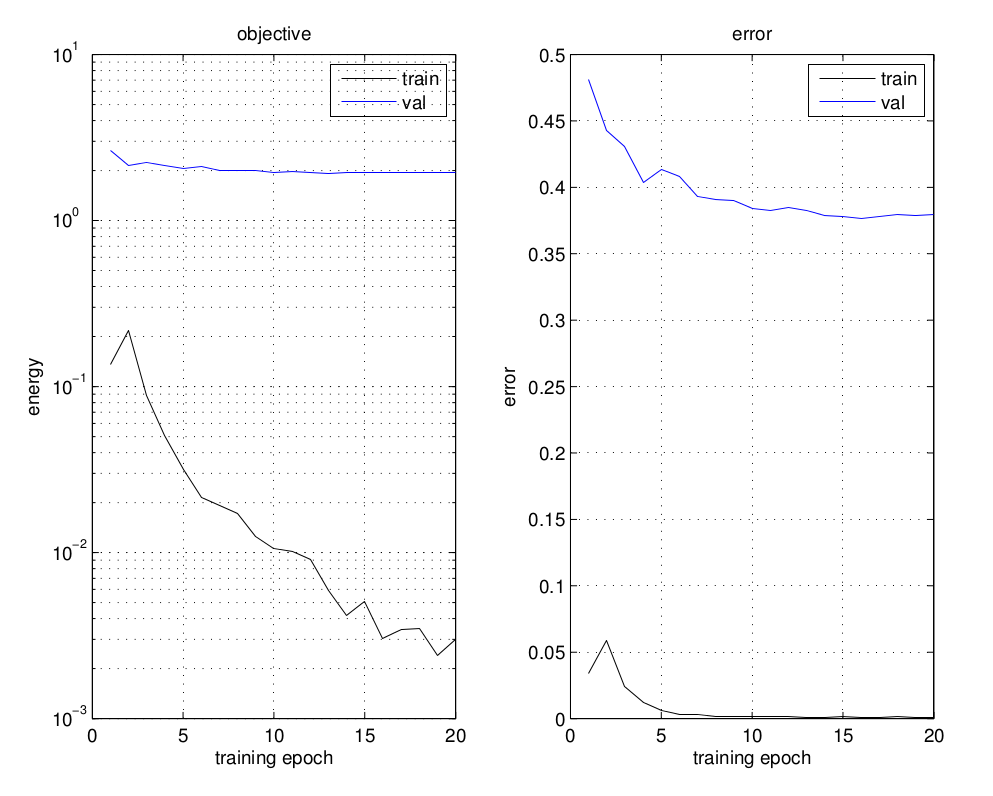
\includegraphics[width=.9\columnwidth]{fig/ft_DAG.png}\label{fig:ft_dag}}

%\caption{Fine-tuning Caffe models on MIT67. The left shows the objectives for training and validation set for each epoch; the right shows the corresponding training and validation error.}
%\label{fig:ft_curve}
%\end{figure}

%{\bf Fine-tuned DAG:} We train a multi-scale DAG-CNN by iterative fine-tuning, making use of a sequence of pre-trained models. We show the results in Fig.~\ref{fig:ft_model}. We begin with off-the-shelf Caffe model. Using a single output layer (as is standard practice) yields a classification accuracy of 59.6\%. Next, we use this model to initialize gradient-based ``fine-tuning'', using training data from MIT-67. This produces a small improvement to 61.7\%. We plot the training and testing accuracy during training epochs in Fig.~\ref{fig:ft_chain}. Finally, we use this fine-tuned chain model to initialize gradient-based learning of a DAG-CNN. To do so, we add multi-scale connections to the chain-structured ``backbone'', as shown in Fig 8 (main paper). The multi-scale weights are initialized to small random numbers, while all other weights in the model are left as-is. End-to-end fine-tuning of our DAG noticeably improves accuracy to 63.5\%. We plot training and testing accuracy during training epochs in Fig.~\ref{fig:ft_dag}. 


%{\bf Off-the-shelf vs. fine-tuned:} 


\begin{figure}[t]
\centering
	\subfigure[SUN397]{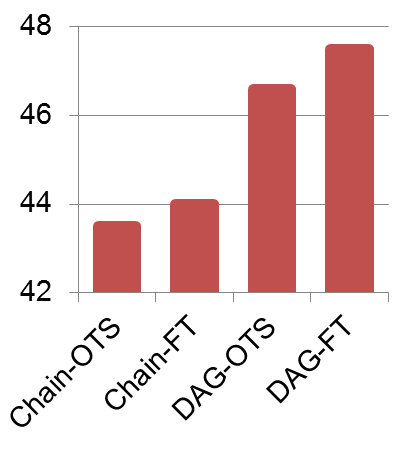
\includegraphics[width=.32\columnwidth]{fig/comp_sun.png}\label{fig:comp_sun}}
	\subfigure[MIT67]{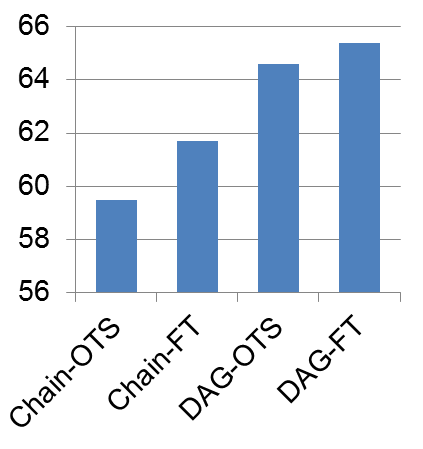
\includegraphics[width=.32\columnwidth]{fig/comp_mit.png}\label{fig:comp_mit}}
	\subfigure[Scene15]{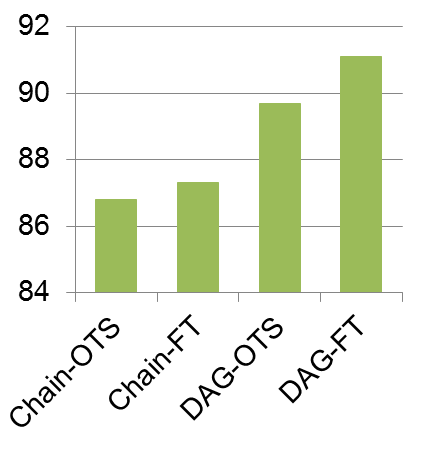
\includegraphics[width=.32\columnwidth]{fig/comp_scene.png}\label{fig:comp_scene}}
	
\caption{Off-the-shelf vs. Fine-tuning models on both Chain and DAG model for Caffe backbone. Please see the text for a discussion.}
\label{fig:comp_otf}
\end{figure}

%
%
%\begin{table}[htbp]
%\begin{center}
%\begin{tabular}{|c|c|c|c|c|}
%\hline
 %& Chain (OTS)  & Chain (FT) &  DAG (OTS) & DAG (FT)\\
%\hline
%SUN397  & 43.5 & 44.0 & 46.6 & 47.5 \\
%MIT67 & 59.5 & 61.7  & 64.6 & 65.4 \\
%Scene15 & 86.8 & 87.3 & 89.7 & 91.1 \\
%\hline
%\end{tabular}
%\end{center}
%\caption{Comparison of chain, off-the-shelf (OTS) , and fine-tuned (FT) models using the Caffe backbone.}
%\label{table:ft_vs_otf}
%\end{table}
%
%{\bf Fine-tuned DAG as feature extractor:} Fine-tuned model can be used as a feature extractor by concatenating features from the DAG model after fine-tuning. This can be viewed as an off-the-shelf feature from multi-scale fine-tune DAG. As compared in Table.~\ref{table:ft_extractor}, when fine-tuned DAG is used as a feature extractor, it is generally better than off-the-shelf multi-scale model with a chain backbone. This demonstrates that fine-tuning procedure encodes more discriminative features at various scales for classification.
%
%\begin{table}[htbp]
%\begin{center}
%\begin{tabular}{|c|c|c|}
%\hline
 %& Deep19-DAG (OTS) &  Deep19-DAG (FT)\\
%\hline
%SUN397 & 55.5 & 56.2 \\
%MIT67 & 76.1 & 77.5 \\
%Scene15 & 92.4 & 92.9 \\
%\hline
%\end{tabular}
%\end{center}
%\caption{Comparison of  and fine-tuned DAG models is used as off-the-shelf feature extractors using the Deep19 backbone. \deva{If we have the nice CAFFE table above, we may not enough need this one.}} 
%\label{table:ft_extractor}
%\end{table}

\begin{figure*}[htbp]
\centering
	\includegraphics[width=\textwidth]{fig/fig_more_eg.png}
\caption{Sample classification results of DAG-CNN model. The category label is shown on the left and the label for false-positives are also provided. \textbf{Top 2 rows:} categories that mid-level features performs better; \textbf{bottom 2 rows:} high-level features does better, shown in Fig.~\ref{fig:level_perf}. The mid-level features emphasize more on \textit{grid texture} for {\tt transition} and \textit{circle} for {\tt laundromat}; the high-level features focus more on global structural statistics.}

\label{fig:more_eg}
\end{figure*}


%-------------------------------------------------------------------------
%-------------------------------------------------------------------------
%\section{Conclusion}

{\bf Conclusion:} We have introduced multi-scale CNNs for image classifcation. Such models encode scale-specific features that can be effectively shared across both coarse and fine-grained classification tasks. Importantly, such models can be viewed as DAG-structured feedforward predictors, allowing for end-to-end training. While fine-tuning helps performance, we empirically demonstrate that even ``off-the-self'' multiscale features perform quite well. We present extensive analysis and demonstrate state-of-the-art classification performance on three standard scene benchmarks, sometimes improving upon prior art by a significant margin. 
{\small
\bibliographystyle{ieee}
\bibliography{mobib}
}

\end{document}
